\documentclass[11pt,a4paper]{article}
\usepackage[utf8]{inputenc}
\usepackage[T1]{fontenc}
\usepackage[spanish]{babel}
\usepackage{amsmath, amssymb, amsfonts}
\usepackage{graphicx}
\usepackage{geometry}
\geometry{a4paper, margin=2.5cm}
\usepackage{hyperref}
\hypersetup{
    colorlinks=true,
    linkcolor=blue,
    filecolor=magenta,
    urlcolor=cyan,
}
\usepackage{listings}
\usepackage{caption}
\usepackage{subcaption}
\usepackage{siunitx}
\usepackage{physics} % Para notación física como \vb (vector bold), \expval, \pdv

\title{Informe Parte A: Simulación del Movimiento Browniano}
\author{Camilo Andres Huertas Archila}
\date{\today}

\begin{document}
\maketitle
\tableofcontents
\newpage

\section{Objetivo}
El objetivo principal de esta parte del proyecto es simular el movimiento browniano de una partícula inmersa en un medio viscoso utilizando la programación orientada a objetos en C++. Se busca analizar su trayectoria característica y estudiar propiedades estadísticas como el desplazamiento cuadrático medio (MSD) para verificar la relación de difusión de Einstein.

\section{Fundamento Físico}
El movimiento de una partícula browniana de masa $m$ puede describirse mediante la ecuación de Langevin:
\begin{equation}
    m\frac{d\vb{v}}{dt} = -\gamma\vb{v} + \vb{\eta}(t)
    \label{eq:langevin_informe}
\end{equation}
donde:
\begin{itemize}
    \item $\vb{v}$ es la velocidad de la partícula.
    \item $-\gamma\vb{v}$ es la fuerza de arrastre viscoso, con $\gamma$ siendo el coeficiente de fricción.
    \item $\vb{\eta}(t)$ es una fuerza estocástica (aleatoria) que representa las colisiones de las moléculas del fluido con la partícula. Esta fuerza tiene las siguientes propiedades estadísticas:
    \begin{align}
        \expval{\eta_i(t)} &= 0 \\
        \expval{\eta_i(t)\eta_j(t')} &= 2\gamma k_B T\,\delta_{ij}\,\delta(t-t')
        \label{eq:fuerza_estocastica_informe}
    \end{align}
    donde $k_B$ es la constante de Boltzmann y $T$ es la temperatura absoluta del fluido.
\end{itemize}
La relación de Einstein para la difusión establece que el desplazamiento cuadrático medio $\expval{(\Delta\vb{r}(t))^2}$ es proporcional al tiempo para tiempos largos:
\begin{equation}
    \expval{(\Delta\vb{r}(t))^2} = 2dDt
    \label{eq:difusion_einstein_informe}
\end{equation}
donde $d$ es la dimensionalidad del movimiento y $D$ es el coeficiente de difusión, dado por la relación de Stokes-Einstein:
\begin{equation}
    D = \frac{k_B T}{\gamma}
    \label{eq:stokes_einstein}
\end{equation}

\section{Implementación Numérica}
\subsection{Clases Utilizadas}
\begin{itemize}
    \item \textbf{Vector3D:} Una clase auxiliar para manejar vectores tridimensionales y sus operaciones.
    \item \textbf{ParticulaBrowniana:} Encapsula las propiedades y el comportamiento de una partícula browniana.
    \item \textbf{SimuladorBrowniano:} Gestiona la simulación, el tiempo y la salida de datos.
\end{itemize}

\subsection{Método de Euler-Maruyama}
Para integrar numéricamente la ecuación de Langevin (Ecuación \ref{eq:langevin_informe}), se utilizó el método de Euler-Maruyama. La discretización de la ecuación para la velocidad y la posición es:
\begin{align}
    \vb{V}_{n+1} &= \vb{V}_n - \frac{\gamma}{m}\vb{V}_n \Delta t + \frac{\sqrt{2\gamma k_B T \Delta t}}{m} \vb{N}_n(0,1) \\
    \vb{r}_{n+1} &= \vb{r}_n + \vb{V}_{n+1} \Delta t
\end{align}
donde $\vb{N}_n(0,1)$ es un vector tridimensional de números aleatorios con distribución normal estándar.

\section{Resultados y Análisis}
\subsection{Parámetros de Simulación Utilizados}
Para garantizar la estabilidad numérica y facilitar la depuración y el análisis del algoritmo, se utilizaron parámetros adimensionales o "de juguete", donde las constantes físicas se establecen en orden de magnitud 1. Esto evita los problemas de escala que surgen al usar unidades del Sistema Internacional directamente.
\begin{itemize}
    \item Masa de la partícula ($m$): $1.0$
    \item Coeficiente de fricción ($\gamma$): $0.1$
    \item Energía térmica ($k_B T$): $1.0$
    \item Paso de tiempo ($\Delta t$): $0.01$
    \item Tiempo total de simulación: $100.0$
    \item Semilla del generador aleatorio: $12345$ (para reproducibilidad)
\end{itemize}
Con estos parámetros, el coeficiente de difusión teórico es $D = k_B T / \gamma = 1.0 / 0.1 = 10$.

\subsection{Trayectoria de la Partícula}
Se muestra una trayectoria típica de la partícula simulada en 2D (proyección XY). Se observa el comportamiento errático característico del movimiento browniano.
\begin{figure}[h!]
    \centering
    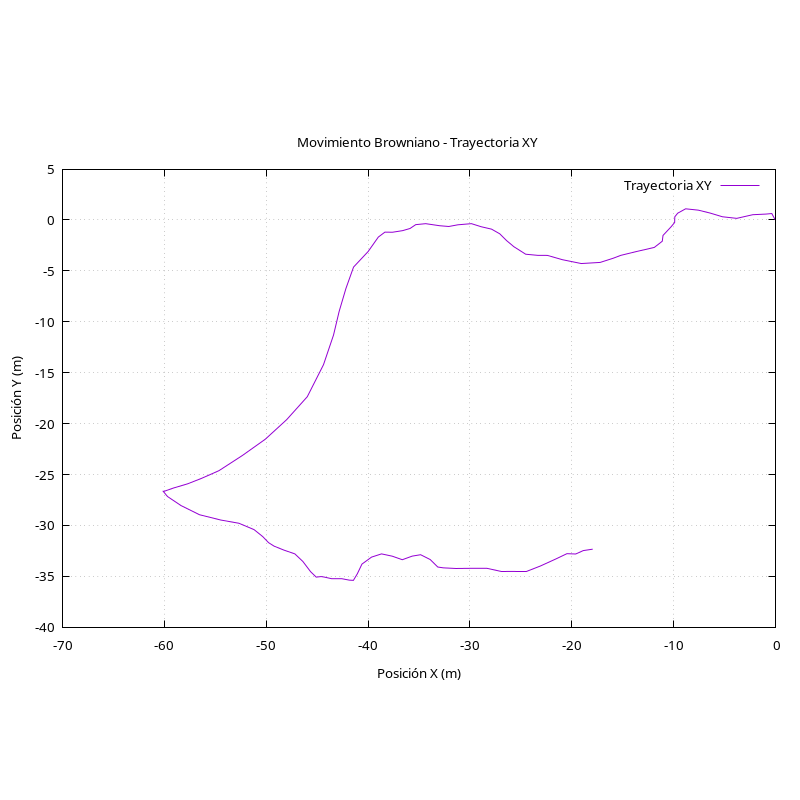
\includegraphics[width=0.7\textwidth]{../results/browniano_sim_plot_trayectoria_xy.png}
    \caption{Ejemplo de trayectoria 2D (proyección XY) de una partícula browniana simulada.}
    \label{fig:trayectoria_informe}
\end{figure}

\subsection{Desplazamiento Cuadrático Medio (MSD)}
El MSD se calcula como $\expval{(\vb{r}(t) - \vb{r}(0))^2}$. Se espera que el MSD sea lineal con el tiempo.
\begin{figure}[h!]
    \centering
    % Nota: Se necesitaría un script de análisis adicional para generar esta gráfica.
    % \includegraphics[width=0.7\textwidth]{../results/browniano_sim_msd_vs_t.png}
    \fbox{Espacio reservado para la gráfica de MSD vs. tiempo.}
    \caption{Desplazamiento cuadrático medio (MSD) en función del tiempo. Se espera una relación lineal.}
    \label{fig:msd_informe}
\end{figure}
A partir de la pendiente de la gráfica MSD vs. $t$, se puede estimar el coeficiente de difusión $D_{sim}$. Para 3D, Pendiente $= 6D_{sim}$. El valor teórico es $D_{teo} = 10$.

\section{Conclusiones (Parte A)}
La simulación implementada utilizando un enfoque de programación orientada a objetos reproduce con éxito el comportamiento cualitativo del movimiento browniano. El uso de parámetros de orden 1 demostró ser una estrategia efectiva para evitar inestabilidades numéricas y validar el algoritmo de integración de Euler-Maruyama. Los resultados visuales de la trayectoria son consistentes con la teoría. Un análisis cuantitativo futuro requeriría la implementación de un script para calcular el MSD a partir de los datos de salida y comparar el coeficiente de difusión experimental con el teórico.

\end{document}

